%Beamer class
\documentclass{beamer}

\usepackage[czech]{babel}
\usepackage[cp1250]{inputenc}
\usepackage{fontenc}
\usepackage{tgheros}
\usepackage{array}

\usetheme{Antibes}
\usecolortheme{crane}


\title[BE1M13VES]{BE1M13VES}
\subtitle[Manufacturing of Electrical Components] {Manufacturing of Electrical Components}
\author[Brejcha]{Michal Brejcha}
\institute[CTU]{CTU in Prague}
\date[Prague, 2017]{Prague, 2017}

\begin{document}
%------------------------------------------------------------------------------
%Uvodni slajd
%------------------------------------------------------------------------------
\frame{\titlepage}

\begin{frame}
\frametitle{Overview} 
\tableofcontents
\end{frame}

\AtBeginSection[]
{
  \begin{frame}
    \frametitle{TOPIC}
    \tableofcontents[currentsection]
  \end{frame}
}
%------------------------------------------------------------------------------
%Terms
%------------------------------------------------------------------------------
\section{\texorpdfstring{Terms}{Terms}}
%------------------------------------------------------------------------------
  \begin{frame}
    \frametitle{Scattering vs Discrete}
		\begin{description}
			\item[Discrete:] 
				\begin{itemize}
					\item The description of the system is given by a specific count of discrete parts (components), that are connected via ideal conductors.
					\item There are only slow changes of the signals. Therefore the time of signal propagation in the system is negligible. The signal level depends only on the time (time is only variable).
				\end{itemize}
			\item[Scattering:]
				\begin{itemize}
					\item The description of the system is given by scattering parameters.
					\item There are fast changes of the signals. The signal propagation depends on time and also on position coordinates in the system.
				\end{itemize}
		\end{description}
  \end{frame}
%------------------------------------------------------------------------------
	\begin{frame}
    \frametitle{Linear vs Nonlinear}
		\begin{description}
			\item[Linear] 
				\begin{itemize}
					\item The system dependency is described only by linear equations.
					\item The superposition can be used.
				\end{itemize}
			\item[Nonlinear] 
				\begin{itemize}
					\item The system dependency is described by nonlinear equations.
					\item They creates other harmonic frequencies for harmonic signals. The superposition cannot be used.
				\end{itemize}
		\end{description}
  \end{frame}
%------------------------------------------------------------------------------
	\begin{frame}
    \frametitle{Passive component vs Active component}
		\begin{description}
			\item[Passive]
				\begin{itemize}
					\item It only dissipates or cumulates the electric energy in electrostatic or magnetic field: resistors, capacitors, inductors, ...
				\end{itemize}
			\item[Active] 
				\begin{itemize}
					\item It contains sources of energy: transistors, amplifiers, sources, ...
				\end{itemize}
		\end{description}
  \end{frame}
%------------------------------------------------------------------------------
%Basic circuit parts
%------------------------------------------------------------------------------
\section{\texorpdfstring{Basic Circuit Components}{Basic Circuit Components}}
%------------------------------------------------------------------------------
	\begin{frame}
    \frametitle{Most Common Circuit Components}
		\begin{center}
			\begin{tabular}{c | c | c | c}
				\hline
				\hline
				\textbf{Component} & \textbf{Symbol} & \textbf{Units} & \textbf{Type} \\
				\hline
			  Voltage source     & 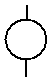
\includegraphics[scale=0.4]{zn_zdrojV.png} & Volts ($V$) & Active\\
				\hline
			  Current source     & 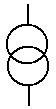
\includegraphics[scale=0.4]{zn_zdrojA.png} & Ampers ($A$) & Active\\
				\hline
			  Resistor     & 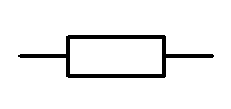
\includegraphics[scale=0.2]{zn_rezistor.png} & Ohms ($\Omega$) & Passive\\
				\hline
			  Kapacitor     & 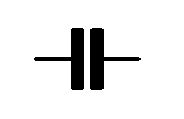
\includegraphics[scale=0.2]{zn_kondenzator.png} & Farads ($F$) & Passive\\
				\hline
			  Inductor     & 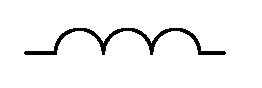
\includegraphics[scale=0.2]{zn_indukcnost.png} & Henry ($H$) & Passive\\
				\hline
				\hline
			\end{tabular}
		\end{center}
  \end{frame}
%------------------------------------------------------------------------------
	\begin{frame}
    \frametitle{Passive Components}
		\begin{center}
		\begin{tabular}{c}
			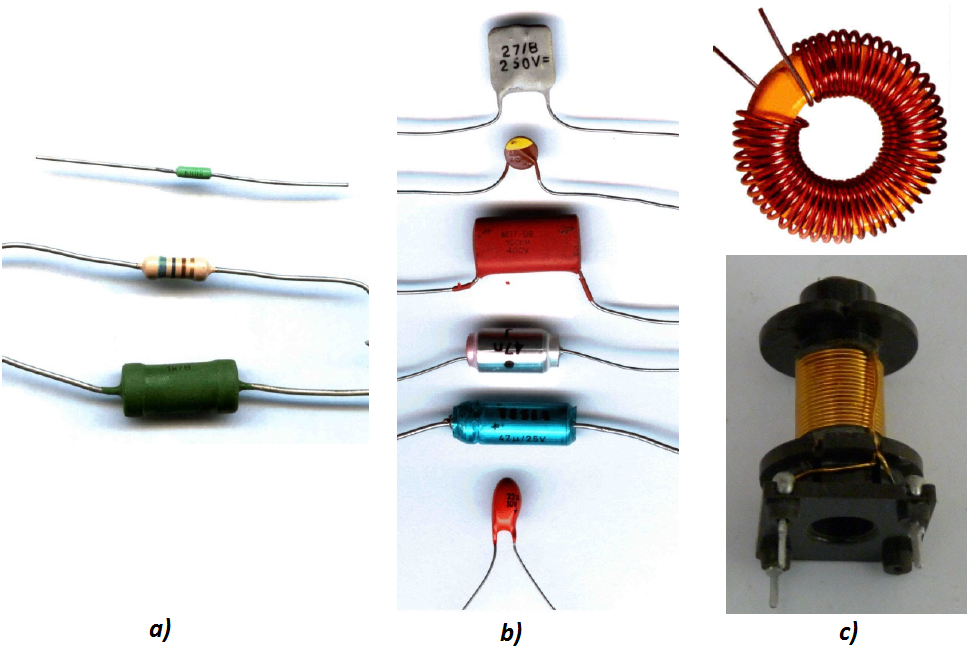
\includegraphics[width=0.8\linewidth]{obr01_RLC.png}\\
			\small{\textit{a)} Resistors, \textit{b)} Capacitors, \textit{c)} Inductors}
		\end{tabular}
		\end{center}
  \end{frame}
%------------------------------------------------------------------------------
	\begin{frame}
    \frametitle{Resistor}
		\begin{center}
		\begin{tabular}{l l}
			\textbf{Basic parameters:} 	& electric resistivity ($R$),\\
																	& dissipated power ($P_{max}$)\\ \\ \hline
			\textbf{Energy:}						& electrical energy $\Rightarrow$ heat\\
																	& $P = u\cdot i = u^2/ R = R\cdot i^2$\\\\
																	& $u$... instantaneous voltage\\
																	& $i$... instantaneous current\\\\ \hline
		  \textbf{Connection:}				& \\
			$R_{total}= \sum{R}$				& $1/R_{total}= \sum{1/R}$\\
			serial											& shunt\\\\
		\end{tabular}
		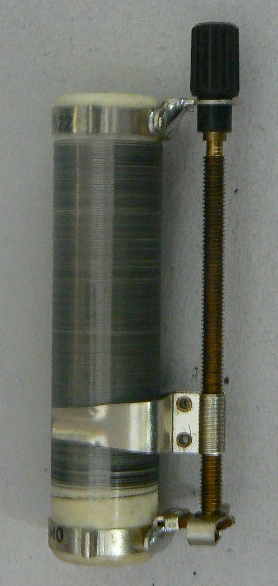
\includegraphics[scale=0.2]{obr02_potenciometr.png}
		\end{center}
  \end{frame}
	
%------------------------------------------------------------------------------
	\begin{frame}
    \frametitle{Ideal Resistor in a Circuit}
		\begin{center}
		\begin{tabular}{m{0.3\linewidth} m{0.6\linewidth}}
			\textbf{Ohms law:} 					& $u\left(t\right)= R\cdot i\left(t\right)$\\\\
			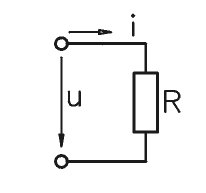
\includegraphics[scale=0.4]{obr03_obvodRez.png}	& 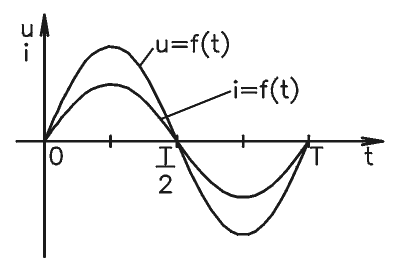
\includegraphics[scale=0.5]{obr04_obvodRezGraf.png}\\
			\textbf{Phasor:}						& $Im\left\{\hat{U}\cdot e^{j\omega t}\right\} = R\cdot Im\left\{\hat{I}\cdot e^{j\omega t}\right\} $\\
																	& $\hat{U} = R\cdot \hat{I}$... $\hat{U}$, $\hat{I}$ no difference in phase
		\end{tabular}
		\end{center}
  \end{frame}
	
%------------------------------------------------------------------------------
	\begin{frame}
    \frametitle{Capacitor}
		\begin{center}
		\begin{tabular}{l l}
			\textbf{Basic parameters:} 	& capacitance ($C$),\\
																	& nominal voltage ($U$)\\ \\ \hline
			\textbf{Energy:}						& electrical energy $\Rightarrow$\\
																	& electrical field\\
																	& $q = C\cdot u$\\
																	& $E = C\cdot u^2/ 2 = q \cdot u/2$\\\\
																	& $u$... instantaneous voltage\\
																	& $q$... instantaneous charge\\\\ \hline
		  \textbf{Connection:}				& \\
			$1/C_{total}= \sum{1/C}$				& $C_{total}= \sum{C}$\\
			serial											& shunt
		\end{tabular}
		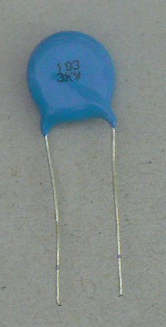
\includegraphics[scale=0.3]{obr05_kondenzator.png}
		\end{center}
  \end{frame}
%------------------------------------------------------------------------------
	\begin{frame}
    \frametitle{Ideal Capacitor in a Circuit}
		\begin{center}
		\begin{tabular}{m{0.3\linewidth} m{0.6\linewidth}}
			\textbf{Current equation:} 					& $i\left(t\right)= C\cdot \frac{\partial u\left(t\right)}{\partial t}$\\\\
			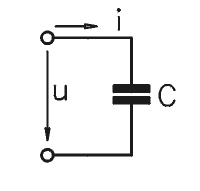
\includegraphics[scale=0.4]{obr06_obvodKond.png}	& 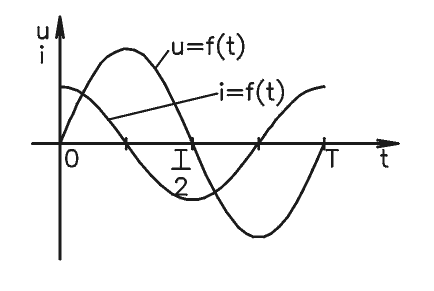
\includegraphics[scale=0.5]{obr07_obvodKondGraf.png}\\
			\textbf{Phasor:}						& $Im\left\{\hat{I}\cdot e^{j\omega t}\right\} = C\cdot \frac{\partial Im\left\{\hat{U}\cdot e^{j\omega t}\right\}}{\partial t}$\\
																	& $\hat{I} = j\omega C \cdot \hat{I}$... $\hat{U}$ is delayed for $90^\circ$ after $\hat{I}$
		\end{tabular}
		\end{center}
  \end{frame}
%------------------------------------------------------------------------------
	\begin{frame}
    \frametitle{Inductor}
		\begin{center}
		\begin{tabular}{l l}
			\textbf{Basic parameters:} 	& inductance ($L$),\\
																	& nominal current ($I$)\\ \\ \hline
			\textbf{Energy:}						& electrical energy $\Rightarrow$\\
																	& magnetic field\\
																	& $\phi = L\cdot i$\\
																	& $E = L\cdot i^2/ 2 = \phi \cdot i/2$\\\\
																	& $i$... instantaneous current\\
																	& $\phi$... instantaneous flux\\\\ \hline
		  \textbf{Connection:}				& \\
			$L_{total}= \sum{L}$				& $1/L_{total}= \sum{1/L}$\\
			serial											& shunt
		\end{tabular}
		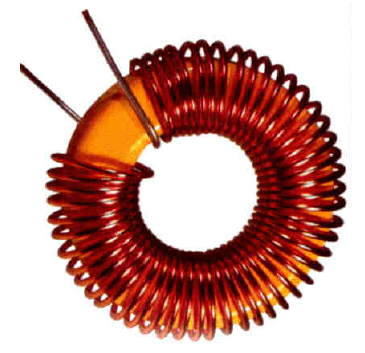
\includegraphics[scale=0.2]{obr08_civka.png}
		\end{center}
  \end{frame}
%------------------------------------------------------------------------------
	\begin{frame}
    \frametitle{Ideal Inductor in a Circuit}
		\begin{center}
		\begin{tabular}{m{0.3\linewidth} m{0.6\linewidth}}
			\textbf{Induced voltage:} 	& $u\left(t\right)= L\cdot \frac{\partial i\left(t\right)}{\partial t}$\\\\
			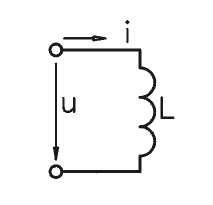
\includegraphics[scale=0.4]{obr09_obvodCiv.png}	& 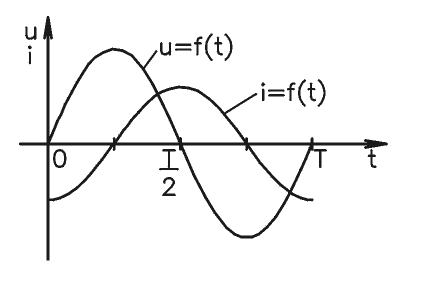
\includegraphics[scale=0.5]{obr10_obvodCivGraf.png}\\
			\textbf{Phasor:}						& $Im\left\{\hat{U}\cdot e^{j\omega t}\right\} = L\cdot \frac{\partial Im\left\{\hat{I}\cdot e^{j\omega t}\right\}}{\partial t}$\\
																	& $\hat{U} = j\omega L \cdot \hat{U}$... $\hat{U}$ is ahead of $\hat{I}$ for $90^\circ$
		\end{tabular}
		\end{center}
  \end{frame}
%------------------------------------------------------------------------------
%Basic circuits
%------------------------------------------------------------------------------
\section{\texorpdfstring{Basic Circuits}{Basic Circuits}}

\end{document}
